\documentclass{beamer}
\usetheme{Madrid}
\usepackage{pifont}
\usepackage{amsmath}
\usepackage{geometry} 
\usepackage{svg}
\usepackage{graphicx}
\usepackage{tikz}

\graphicspath{ {./assets/} }
\usetikzlibrary{positioning}
\usetikzlibrary{shapes.geometric, arrows.meta, positioning, fit, calc, backgrounds}

% Define Colors based on your Mermaid Graph
\definecolor{colInput}{HTML}{E1F5FE}
\definecolor{strokeInput}{HTML}{01579B}
\definecolor{colProcess}{HTML}{F3E5F5}
\definecolor{strokeProcess}{HTML}{4A148C}
\definecolor{colModel}{HTML}{FFF3E0}
\definecolor{strokeModel}{HTML}{E65100}
\definecolor{colDecision}{HTML}{FFF9C4}
\definecolor{strokeDecision}{HTML}{FBC02D}
\definecolor{colOutput}{HTML}{E8F5E9}
\definecolor{strokeOutput}{HTML}{1B5E20}


\title{Few-Shot Code Forensics: Detecting AI-Generated Code using UniXcoder Prototypical Networks}
\author{Arif Akbarul Huda  (25/571619/SPA/01156) }

\begin{document}
	\begin{frame}
		\titlepage
	\end{frame}
	\begin{frame}
		\frametitle{The Datasets}
		\begin{figure}
			\centering
			\includegraphics[height=0.5 \linewidth]{human_vs_ai_distribution.png}
			\caption{The distribution human vs ai accross training, validation, test}			
		\end{figure}
	\end{frame}
	\begin{frame}
		\frametitle{The Datasets}
		\begin{figure}
			\centering
			\includegraphics[height=0.50 \linewidth]{snippet_code.png}
			\caption{The example human vs ai generated code}			
		\end{figure}
	\end{frame}

	\begin{frame}
		\frametitle{The Datasets}
		\begin{figure}
			\centering
			\includegraphics[width=0.80 \linewidth]{table_summaries_data.png}
			\caption{The datasets summarize across training, validation, test}			
		\end{figure}
	\end{frame}
	\begin{frame}
	\frametitle{ARCHITECTURE AND TRAINING STRATEGY}
		\framesubtitle{Model Architecture}
		\begin{itemize}
			\item  microsoft/unixcoder-base, a pre-trained cross-lingual model suitable for code representation.
			\item  Prototypical Network (Metric-based Meta-Learning).
			\item  Projects code samples into a metric space and classifies them based on Euclidean distance to class prototypes (Human vs. AI)
		\end{itemize}
	\end{frame}
	\begin{frame}
		\frametitle{ARCHITECTURE AND TRAINING STRATEGY}
		\framesubtitle{Training Strategy - Episodic Meta-Training}
		\begin{itemize}
			\item  Training simulates "N-Way, K-Shot" tasks (N=2 classes, K=5 support samples, Q= 30)
			\item  AdamW optimizer with learning rate decay
			\item  HIDDEN DIM = 768 , Q QUERY = 30
		\end{itemize}
	\end{frame}
	\begin{frame}
		\frametitle{ARCHITECTURE AND TRAINING STRATEGY}
		\framesubtitle{Training Strategy - Test Time Adaptation}
		\begin{itemize}
		\item  Pseudo-Labeling
		\item  Transductive Fine-tuning
		\end{itemize}
	\end{frame}
	\begin{frame}{ML Pipeline: Meta-Training \& Adaptation}
		\centering
		% FIX: Scale based on height (0.85\textheight) to fit slide vertically.
		% The '!' for width allows it to adjust automatically to maintain aspect ratio.
		\resizebox{!}{0.85\textheight}{%
			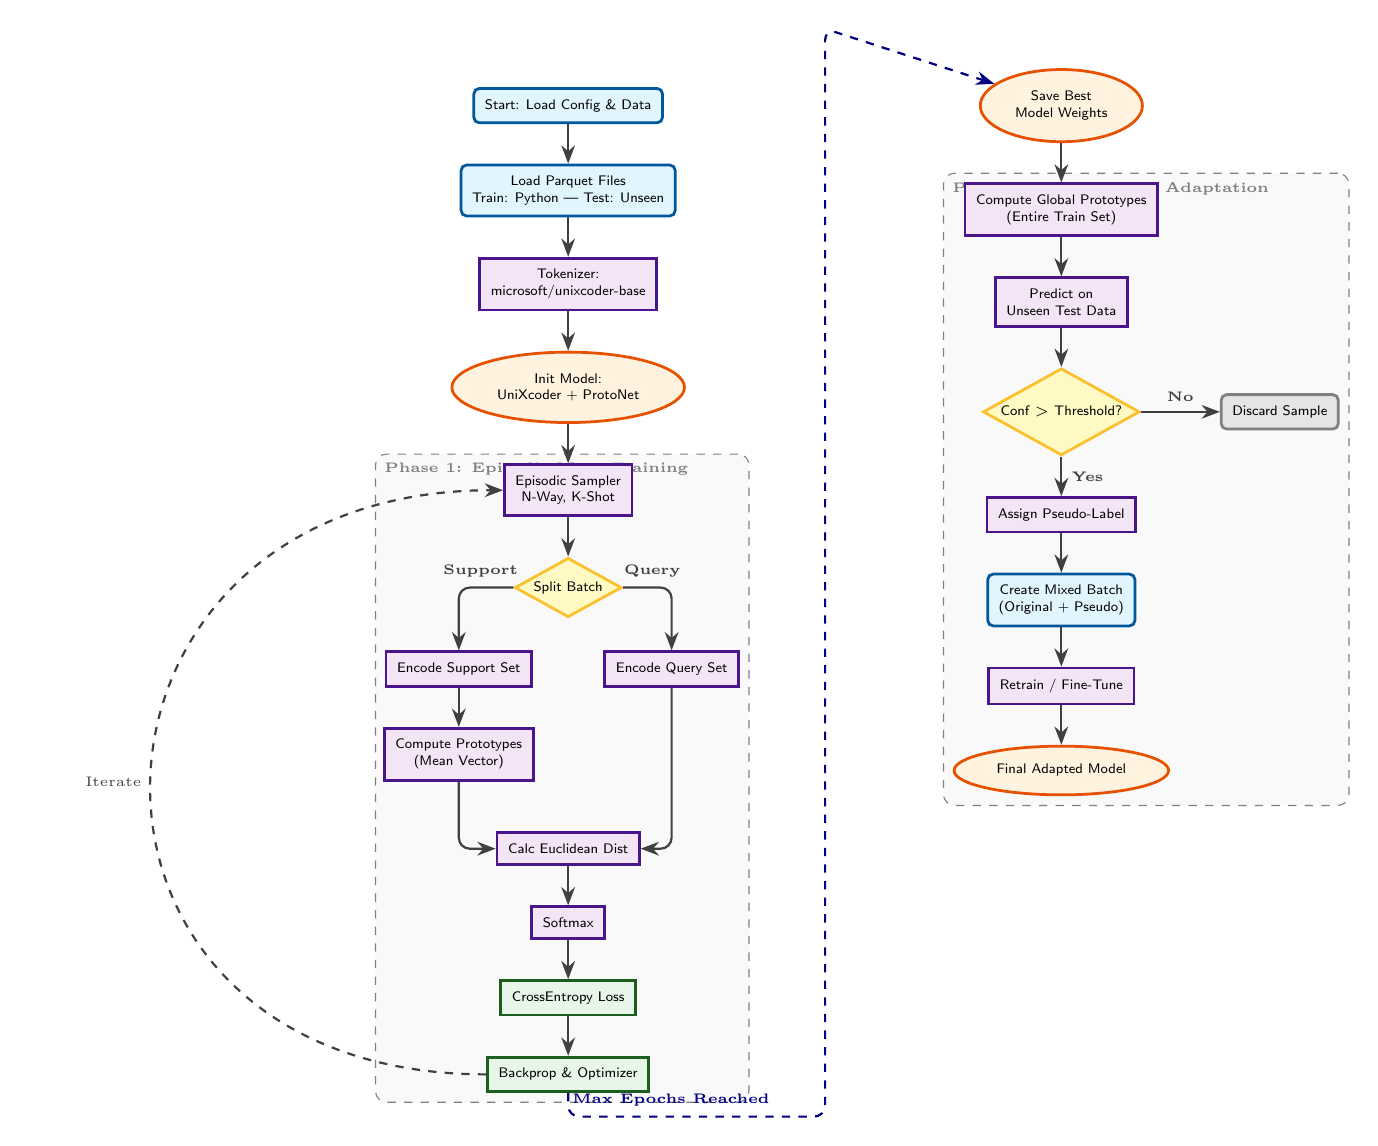
\begin{tikzpicture}[
				node distance=0.5cm and 0.4cm, % Slightly tighter spacing
				font=\sffamily\tiny,
				% Node Styles
				base/.style={draw, line width=1pt, align=center, inner sep=4pt},
				input/.style={base, fill=colInput, draw=strokeInput, rounded corners=2pt, rectangle},
				process/.style={base, fill=colProcess, draw=strokeProcess, rectangle},
				model/.style={base, fill=colModel, draw=strokeModel, ellipse},
				decision/.style={base, fill=colDecision, draw=strokeDecision, diamond, aspect=1.8, inner sep=1pt},
				output/.style={base, fill=colOutput, draw=strokeOutput, rectangle},
				arrow/.style={-Stealth, thick, rounded corners, darkgray}
				]
				
				%% ================= COLUMN 1: PHASE 1 =================
				\node[input] (start) {Start: Load Config \& Data};
				\node[input, below=of start] (dataload) {Load Parquet Files\\Train: Python | Test: Unseen};
				\node[process, below=of dataload] (tokenizer) {Tokenizer:\\microsoft/unixcoder-base};
				\node[model, below=of tokenizer] (initmodel) {Init Model:\\UniXcoder + ProtoNet};
				
				\node[process, below=of initmodel] (sampler) {Episodic Sampler\\N-Way, K-Shot};
				\node[decision, below=of sampler] (split) {Split Batch};
				
				% Branches
				\node[process, below left=0.6cm and 0.1cm of split] (suppenc) {Encode Support Set};
				\node[process, below right=0.6cm and 0.1cm of split] (queryenc) {Encode Query Set};
				
				\node[process, below=of suppenc] (prototypes) {Compute Prototypes\\(Mean Vector)};
				
				% Merge Node Positioning
				\node[process] (distcalc) at ($(split |- prototypes) + (0, -1.2)$) {Calc Euclidean Dist};
				
				\node[process, below=of distcalc] (softmax) {Softmax};
				\node[output, below=of softmax] (loss) {CrossEntropy Loss};
				\node[output, below=of loss] (backprop) {Backprop \& Optimizer};
				
				% Edges Col 1
				\draw[arrow] (start) -- (dataload);
				\draw[arrow] (dataload) -- (tokenizer);
				\draw[arrow] (tokenizer) -- (initmodel);
				\draw[arrow] (initmodel) -- (sampler);
				\draw[arrow] (sampler) -- (split);
				\draw[arrow] (split) -| node[pos=0.3, above, font=\tiny\bfseries] {Support} (suppenc);
				\draw[arrow] (split) -| node[pos=0.3, above, font=\tiny\bfseries] {Query} (queryenc);
				\draw[arrow] (suppenc) -- (prototypes);
				
				% Merge Connections
				\draw[arrow] (prototypes) |- (distcalc);
				\draw[arrow] (queryenc) |- (distcalc);
				
				\draw[arrow] (distcalc) -- (softmax);
				\draw[arrow] (softmax) -- (loss);
				\draw[arrow] (loss) -- (backprop);
				
				% Loop Back (Left Side)
				\draw[arrow, dashed] (backprop.west) to[out=180,in=180, looseness=2] node[left, font=\tiny, align=right] {Iterate} (sampler.west);
				
				%% ================= COLUMN 2: PHASE 2 =================
				\node[model, right=4cm of start] (savemodel) {Save Best\\Model Weights};
				
				% Transition Line
				\draw[arrow, blue!50!black, dashed] (backprop.south) -- ++(0,-0.3) -| node[pos=0.2, above, font=\bfseries\tiny] {Max Epochs Reached} ($(savemodel.north) + (-3, 0.5)$) -- (savemodel);
				
				\node[process, below=of savemodel] (globalproto) {Compute Global Prototypes\\(Entire Train Set)};
				\node[process, below=of globalproto] (predict) {Predict on\\Unseen Test Data};
				\node[decision, below=of predict] (confidence) {Conf $>$ Threshold?};
				
				\node[process, below=of confidence] (pseudo) {Assign Pseudo-Label};
				\node[input, right=1.0cm of confidence, fill=gray!20, draw=gray] (discard) {Discard Sample};
				
				\node[input, below=of pseudo] (mixed) {Create Mixed Batch\\(Original + Pseudo)};
				\node[process, below=of mixed] (finetune) {Retrain / Fine-Tune};
				\node[model, below=of finetune] (final) {Final Adapted Model};
				
				% Edges Col 2
				\draw[arrow] (savemodel) -- (globalproto);
				\draw[arrow] (globalproto) -- (predict);
				\draw[arrow] (predict) -- (confidence);
				\draw[arrow] (confidence) -- node[right, font=\tiny\bfseries] {Yes} (pseudo);
				\draw[arrow] (confidence) -- node[above, font=\tiny\bfseries] {No} (discard);
				\draw[arrow] (pseudo) -- (mixed);
				\draw[arrow] (mixed) -- (finetune);
				\draw[arrow] (finetune) -- (final);
				
				%% ================= BACKGROUNDS =================
				\begin{scope}[on background layer]
					\node[fit=(sampler)(backprop)(queryenc)(suppenc), fill=gray!5, draw=gray, dashed, rounded corners, label={[anchor=north west, gray, font=\tiny\bfseries]north west:Phase 1: Episodic Meta-Training}] (phase1) {};
					\node[fit=(globalproto)(final)(discard), fill=gray!5, draw=gray, dashed, rounded corners, label={[anchor=north west, gray, font=\tiny\bfseries]north west:Phase 2: Self-Training Adaptation}] (phase2) {};
				\end{scope}
				
			\end{tikzpicture}
		}
	\end{frame}
	\begin{frame}
	\frametitle{Validation Report}
	\begin{figure}
		\centering
		\includegraphics[width=1 \linewidth]{poster2.png}
		\caption{The metric on validation data}			
	\end{figure}
	\end{frame}
	\begin{frame}
	\frametitle{Test Report}
	\begin{figure}
		\centering
		\includegraphics[width=1 \linewidth]{poster3.png}
		\caption{The metric on test data}			
	\end{figure}
	\end{frame}
	\begin{frame}
	\frametitle{Test Report}
	\begin{figure}
		\centering
		\includegraphics[width=1 \linewidth]{poster1.png}
		\caption{The metric on test data after self adaption}			
	\end{figure}
	\end{frame}
	\begin{frame}
	\frametitle{Test Report}
	\begin{figure}
		\centering
		\includegraphics[width=1 \linewidth]{poster4.png}
		\caption{The model performance comparison}			
	\end{figure}
	\end{frame}

	\begin{frame}
		\frametitle{Sem-eval 2026 Competition}
		\framesubtitle{Per 5 Dec 2025 - on going}
		\begin{itemize}
			\item  218 Entrants
			\item  106 Participants
			\item  97 Teams
			\item  826 Submissions
		\end{itemize}
	\end{frame}
	\begin{frame}
		\frametitle{Sem-eval 2026 Submission}	% Begin the columns environment
		
		% 1. TOP ROW: TWO COLUMNS (50% each)
		\begin{columns}
			% --- Left Column (Row 1, Col 1) ---
			\begin{column}{0.48\textwidth}
				\centering
				\includegraphics[width=0.9\linewidth]{1st_submission.png}
				\footnotesize{14Nov2025}
			\end{column}
			
			% --- Right Column (Row 1, Col 2) ---
			\begin{column}{0.48\textwidth}
				\centering
				\includegraphics[width=0.9\linewidth]{2nd_submission.png}
				\footnotesize{28Nov2025}
			\end{column}
		\end{columns}
		
		% Optional: Add a small vertical space between the rows
		\vspace{0.5em}
		\hrule % Optional: A horizontal line to visually separate the rows
		
		% 2. BOTTOM ROW: ONE MERGED COLUMN
		% We use \vfill to push the content to the bottom and a minipage to control its width
		\vfill 
		\begin{minipage}{\textwidth} % Minipage spans the full text width
			\centering
			
			\begin{figure}
				\centering
				\includegraphics[width=1 \linewidth]{3rd_submission.png}
				\footnotesize{4Dec2025}			
			\end{figure}
		\end{minipage}
		
	\end{frame}
\end{document}